% interactnlmsample.tex
% v1.05 - August 2017

\documentclass[]{interact}

\usepackage{epstopdf}% To incorporate .eps illustrations using PDFLaTeX, etc.
\usepackage[caption=false]{subfig}% Support for small, `sub' figures and tables
%\usepackage[nolists,tablesfirst]{endfloat}% To `separate' figures and tables from text if required
%\usepackage[doublespacing]{setspace}% To produce a `double spaced' document if required
%\setlength\parindent{24pt}% To increase paragraph indentation when line spacing is doubled

\usepackage{tikz}

\usepackage{pdfpages}
\usepackage{pgfplots}
\usepackage{enumerate}
\usepackage{verbatim}
\usepackage{dirtytalk}
\usepackage{caption}
\captionsetup{
  justification = centering
}


\usepackage[numbers,sort&compress]{natbib}% Citation support using natbib.sty
\bibpunct[, ]{[}{]}{,}{n}{,}{,}% Citation support using natbib.sty
\renewcommand\bibfont{\fontsize{10}{12}\selectfont}% Bibliography support using natbib.sty
\makeatletter% @ becomes a letter
\def\NAT@def@citea{\def\@citea{\NAT@separator}}% Suppress spaces between citations using natbib.sty
\makeatother% @ becomes a symbol again

\theoremstyle{plain}% Theorem-like structures provided by amsthm.sty
\newtheorem{theorem}{Theorem}[section]
\newtheorem{lemma}[theorem]{Lemma}
\newtheorem{corollary}[theorem]{Corollary}
\newtheorem{proposition}[theorem]{Proposition}

\theoremstyle{definition}
\newtheorem{definition}[theorem]{Definition}
\newtheorem{example}[theorem]{Example}

\theoremstyle{remark}
\newtheorem{remark}{Remark}
\newtheorem{notation}{Notation}

\begin{document}

\articletype{ARTICLE TEMPLATE}% Specify the article type or omit as appropriate

\title{Evolving Planet Wars bots: Artificial immune system against Particle swarm optimization}

\author{
\name{C.~T. Mohamed-Amine\textsuperscript{a}\thanks{CONTACT C.~T. Mohamed-Amine. Email: ma\_chikhtouhami@hotmail.com} , Salem Mohammed\textsuperscript{b} and Khelfi Mohammed Faycel\textsuperscript{c}}
\affil{\textsuperscript{a}Chikh Touami Mohamed Amine, Faculty of Exact Science, University Mustafa Stembouli, Mascara, Algeria; \textsuperscript{b}Faculty of Exact Science, University Mustafa Stembouli, Mascara, Algeria; \textsuperscript{c}RIIR Lab, University of Oran 1, Oran, Algeria;}
}

\maketitle

\begin{abstract}
Inherited by the real-time aspect, one of the hardest tasks in RTS games is the designing of the agents(Bots).within the Planetwar game, the bot need a set of parameters that will determine the actions to perform during the playing match. In this work, we present two evolving approaches based on evolutionary computational methods that will be applied to improve the behavior of the Planet Wars bot. The first one uses the artificial immune system while the second one take advantage from the strength of the particle swarm intelligence to tune these parameters. The evolving approaches yield good results when  evaluated and compared to genetic algorithms.
\end{abstract}

\begin{keywords}
Computational intelligence, real-time strategy
games, planet wars, artificial immune system, particle swarm optimization.
\end{keywords}


\section{Introduction}
% no \IEEEPARstart
\paragraph*{} 
Nowadays, there has been an increasing interest in the field of video games. The influence of these video games in our life and culture led the researchers to try to design more realistic games for more entertainment. On the other hand, there is more than one kind of video games, such as chess, go, non-player character (NPC) and first
person shot (FPS) to mention a few. 
\paragraph*{} 
In this study, we interested in a different subgenre of video games called strategy video games. in this kind of games you have to control a set of units distributed on a multidimensional space when contenders have to move in the aim of destroying all the enemies structures in the minimum number of turns or to protect the self-unit till the end without losing the game. those games, by their nature, are real-time games, that mean all players have to act simultaneously without waiting other to move\cite{doc3} like chess or go. \par 
Existing research in real-time strategy games (RTS) recognizes the critical role played by computational intelligence in this major. Moreover, inherited by their nature, RTS games are a good tool for testing the different methods and technics of computational by creating new challenges to improve the designing process of this kind of games. In the other side, the contribution of Computational in that genre of games lies in the conception of the agent that will play the game and interact with the human side.\cite{doc5,doc1,doc2,doc3,doc4}

\paragraph*{}
this research focuses on one of the RTS games called Planet Wars. In this game, two players will be faced on multiple types of maps in the aim of overwhelmed the opponent or to protect the self-units without losing the game. While Each player can generate multiple attacks against the other contenders including a specific number of troops in several strategies to bit the enemy. Moreover, the players on our case are autonomous agents that will react in a real scenario under this game, those agents named Bot. As we mentioned previously, one of the most challenges in RTS games is the Bot conception. This intelligent agent will act under a computer-based framework\cite{doc3} against a human player in order to compete it.

\paragraph*{}
The Bot conception is a major area of interest\cite{doc4} within the field of computational intelligence in order to design an RTS game. Which, the problem is the real-time aspect related to this type of games. In addition, to control a Planet Wars agent, a set of parameters previously improved will determine the reaction of the Bot under the game. Among all Planet Wars parameters, we have to choose a set of the highly effective ones\cite{doc5} that will be used by the Bot for best behavior during the game.\par
This process already an optimization issue\cite{doc5}, whilst, our work is to improve some parameters predefined by experts in the domain. So, the optimization process will move in three fields: the first step is going by using an algorithm inspired by the immune system of the human body called an Artificial Immune System (AIS). The second step is to run another nature-inspired algorithm named Particle Swarm Optimization (PSO), this algorithm behaves in the same way with nature animals swarms as bird swarms, fish schooling ...etc. The last step is to make a comparison between those two optimization methods and the one used in\cite{doc1} that implemented the Genetic Algorithm (GA).

\paragraph*{}
This paper begins by describing Planet Wars, the game used in this work and all the rule related to. It will then go on to explain the AIS and PSO algorithms and how it works. The third part is about the general based architecture of the bot to move intelligently during the game. The last section tries to define the comparable results between the optimization methods used.

\section{Planet Wars}

As we mentioned previously one of the international competition was organized by google community. In this pager, we worked with planet war game chosen as RTS game in this competition with the aim of designing a fighter bot. During a planet war\cite{doc1}, firstly you have to choose a map to run a match, each map has a number of distributed planets in different positions with a specific number emerged the starships amount situated in the planet\cite{lucas}. Each planet in the map owned by player, opponent or neutral (owned by no one), moreover, each planet owner by players will increase the number starship per turn based on their growth rate except the neutral planets that will not be able to generate new additional starships. The main purpose of planet war\cite{doc1} is to compete with other players and try to beat all of them during the game by limited turns number.  \\

Moreover, the planet war fighter bot face two important problems that make the agent's conception more challenging:
The first problem \cite{doc1} that the bot can bot save any previous stats from previous turns as actions it made, map state...etc. Since in each turn, bot finds under an unknown map the same thing when it begins the game in the first time. The second problem\cite{doc3} in inherited by the RTS game nature that is shown as the time required to act (make an action) is defined by 1 second.

\begin{figure}
\centering
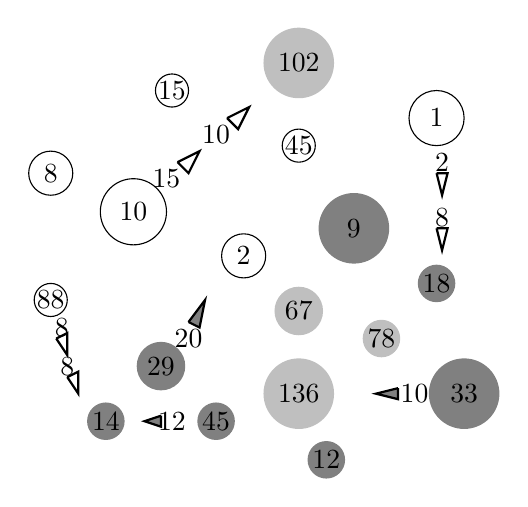
\begin{tikzpicture}[scale = 0.7]
\draw [fill =gray, ultra thick, gray] (2,1) circle [radius=0.3];
\node at (2,1) {14};
\draw [fill =gray, ultra thick, gray] (3,2) circle [radius=0.4];
\draw [fill = gray ,thick] (3.5,2.8) to (3.7,2.7) to (3.8,3.2) to (3.5,2.8);
\node at (3.5,2.5) {20};
\node at (3,2) {29};
\draw [fill =gray, ultra thick, gray] (4,1) circle [radius=0.3];
\node at (4,1) {45};
\draw [fill =gray ,thick] (3,1.1) to (3,0.9) to (2.7,1) to (3,1.1);
\node at (3.2,1) {12};
\draw [fill =gray, ultra thick, gray] (6,0.3) circle [radius=0.3];
\node at (6,0.3) {12};
\draw [fill =gray, ultra thick, gray] (8.5,1.5) circle [radius=0.6];
\node at (8.5,1.5) {33};
\draw [fill = gray ,thick] (7.3,1.6) to (6.9,1.5) to (7.3,1.4) to (7.3,1.6);
\node at (7.6,1.5) {10};
\draw [fill =gray, ultra thick, gray] (8,3.5) circle [radius=0.3];
\node at (8,3.5) {18};
\draw [fill =gray, ultra thick, gray] (6.5,4.5) circle [radius=0.6];
\node at (6.5,4.5) {9};
%\draw [fill =lightgray, ultra thick, lightgray] (3.5,3) circle [radius=0.3];
%\node at (3.5,3) {78};
\draw [fill =lightgray, ultra thick, lightgray] (5.5,1.5) circle [radius=0.6];
\node at (5.5,1.5) {136};
\draw [fill =lightgray, ultra thick, lightgray] (5.5,3) circle [radius=0.4];
\node at (5.5,3) {67};
\draw [fill =lightgray, ultra thick, lightgray] (7,2.5) circle [radius=0.3];
\node at (7,2.5) {78};
\draw [fill =lightgray, ultra thick, lightgray] (5.5,7.5) circle [radius=0.6];
\node at (5.5,7.5) {102};
\draw (1,3.2) circle [radius=0.3];
\node at (1,3.2) {88};
\draw [thick] (1.1,2.5) to (1.3,2.6) to (1.3,2.2) to (1.1,2.5);
\draw [thick] (1.3,1.8) to (1.5,1.9) to (1.5,1.5) to (1.3,1.8);
\node at (1.2,2.7) {8};
\node at (1.3,2) {8};
\draw  (1,5.5) circle [radius=0.4];
\node at (1,5.5) {8};
\draw  (2.5,4.8) circle [radius=0.6];
\node at (2.5,4.8) {10};
\draw  (3.2,7) circle [radius=0.3];
\draw [thick] (3.3,5.7) to (3.7,5.9) to (3.5,5.5) to (3.3,5.7);
\draw [thick] (4.2,6.5) to (4.6,6.7) to (4.4,6.3) to (4.2,6.5);
\node at (3.1,5.4) {15};
\node at (4,6.2) {10};
\node at (3.2,7) {15};
\draw  (4.5,4) circle [radius=0.4];
\node at (4.5,4) {2};
\draw  (5.5,6) circle [radius=0.3];
\node at (5.5,6) {45};
\draw  (8,6.5) circle [radius=0.5];
\draw [thick] (8,5.5) to (8.2,5.5) to (8.1,5.1) to (8,5.5);
\draw [thick] (8,4.5) to (8.2,4.5) to (8.1,4.1) to (8,4.5);
\node at (8,6.5) {1};
\node at (8.1,5.7) {2};
\node at (8.1,4.7) {8};
\end{tikzpicture}
\caption{an early stage of a planet wars game, as shown here there are planet categories, the darker grey (red in the game) ones related to the player, the white ones (green in the game) related to the opponent and the neutral planets are coloured by light grey. Fleets presented by triangles and the numbers are the starships included on them.}
\end{figure}

The environment of planet war forced to assign properties to every single object in the game.\cite{doc1} Such as, each planet in the map has two coordination points X and Y for its location, the ownerID, number of troops situated on it and the growth rate. To make an attack against enemies, the bot has to include starships and fleets under the attack. Each fleet has playerID, starships number included on it, source planetID, destination planetID and the number of turns need to achieve the goal, While the player is able to make one action per turn.\cite{doc1}

After each action, the planets will increase their ships number based on their growth rate.\cite{doc5, lucas} Moreover, if the source planet and the destination planet owner are the same ones, so we will consider that as a reinforcement by adding extra ships to the destination planet. Otherwise, if the target is a neutral planet, the bot has to calculate the exact starships need to win conquest the planet, whilst, if the target is an opponent, the two contenders will fight until one of them who has the highest number of starships will win the planet.\cite{doc1,doc5}

When the player makes an action and sends fleets, they can not change their direction until they will reach the destination they sent for it. As we mentioned previously, each match has a limited number of turns cannot go throw. So, by the end of the match, the player with the highest number of ships win the game. If one of them lose all their ships without finishing their total turns number, the game will complete faster, whilst, if the two players have the same number of troops, we have a draw.\cite{doc5}. 
\section{immune system overview}
The biology is one of the most inspirational domains that help the computational to solve many hard problems.\cite{doc7} Among the natural concepts, the immune system is one of the important aspects that provide several technics to design many optimization algorithms. An optimization problem\cite{doc6} is to search for the optimum solution from a set of potential solutions. The most algorithms used in this wide research are Heuristics.\cite{doc6} That include divers algorithms such as firefly swarm optimization, artificial bee colony, genetic algorithm, just to mention a few. While the Artificial Immune system (AIS)\cite{doc6} is a population-based algorithm. However, the application of the Artificial Immune System within technologies areas is a challenge is a self. Likewise, the researchers could exploit just a few immune's mechanisms because even in biology, this system still under a wide research area itself. 

\subsection{natural immune system}
The biological immune system including human system contains cells, molecules, and organs in the global structure to defend the body against diseases.\cite{doc6} The immune system has the ability to recognize the self-body cells and the nonself cells. In addition, this technic is very important to make an immune response by activating a suitable process to defeat the nonself cells.\cite{doc6} This response process will be activated according to antigens type, every antigene type activate a specific immune response process. whilst, memory cells are produced and activate when there is the same immune response type later.
\subsubsection*{Clonal selection}
To activate a response against the pathogens, the immune system uses multiple mechanisms. One of the interesting immune response is the clonal selection, this response type describes the process how the immune system can stimulus against a specific type of pathogens by proliferating a specific type of cells who can recognize the antigen.\cite{doc7} When a clonal selection response was stimulated, a specific type of cells (the B-cells) be proliferating according to affinity maturation, that's mean the high affinity will generate a hight clone number.
\begin{figure}
\centering
\begin{tabular}{c}
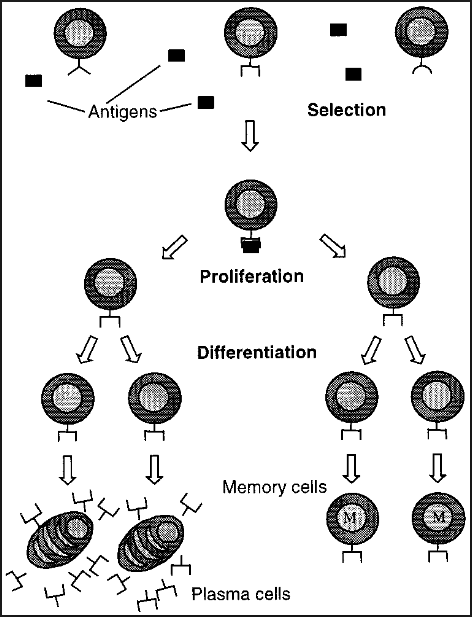
\includegraphics[scale = 0.6]{clonaS}
\end{tabular}
\caption{The biological clonal selection mechanism and its steps in order to defend the body, starting by detecting of the antigen until removing it.}
\end{figure}
The clonel selection process pass with multiple stps:
\begin{enumerate}
\item[--] The cloned cells undergo to a mutation process.
\item[--] the self-reactive receptor will be eliminated.
\item[--] proliferate the mature cells those can detect the antigen.
\end{enumerate} 
\subsection{Artificial Immune System}
In light of recent event in AIS, many algorithms have been developed trying to simulate ti clonal selection process. In 2002 Castro and Zuben proposed an optimization algorithm named CLONALG. The first step of this algorithm is to initialize an N random antibodies present the N potential solutions. in each iteration, the antibodies are cloned, mutated and selected the best of them preparing for the next generation. The proliferation of the antibodies is according to their affinities. While the maturation applied to equation (1): 
\begin{equation}
x_{id} = x_{id} + k(x_{d_{max}} - x_{d_{min}}) . N(0,1)
\end{equation}
where $x_{id}$ represent the dimension d of the antibody i, $x_{max}$ and $x_{min}$ represent the min and the max bounds of the variable i, N(0,1) is the standard distribution and k is the scale factor.

New random antibodies will be added to the original population by replacing a percentage of worsting antibodies and preparing to next generation.
\subsection{AIS pseudocode}
\begin{enumerate}
\item initialize N individual with random values between 0 and 1.
\item For iteration = 1 : maxIteration,
\begin{itemize}
\item Compute the affinities.
\item Clone the antibodies.
\item Mutate the antibodies cloned in the previous step.
\item Compute the affinities for the new antibodies mutated.
\item Applied the selection process to select the next generation
\end{itemize} 
End For \\
Display the optimal solutions. \\
End
\end{enumerate}
\begin{figure}[t]
\centering
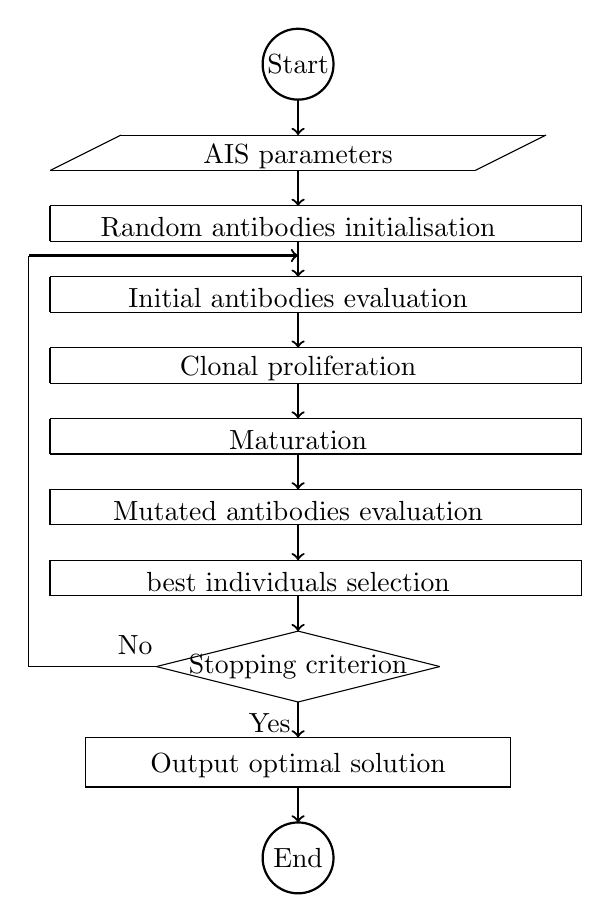
\begin{tikzpicture}[scale = 0.9]
\draw [thick] (4.5,20) circle [radius=0.5];
\node at (4.5,20) {Start};
\draw [->] [thick](4.5,19.5) -- (4.5,19);
\draw (2,19) --(8,19);
\draw (1,18.5) --(7,18.5);
\draw (2,19) --(1,18.5);
\draw (8,19) --(7,18.5);
\node at (4.5,18.7) {AIS parameters};
\draw [->] [thick](4.5,18.5) -- (4.5,18);
\draw (1,18) --(8.5,18);
\draw (1,17.5) --(8.5,17.5);
\draw (1,18) --(1,17.5);
\draw (8.5,18) --(8.5,17.5);
\node at (4.5,17.7) {Random antibodies initialisation};
\draw [->] [thick](4.5,17.5) -- (4.5,17);
\draw (1,17) --(8.5,17);
\draw (1,16.5) --(8.5,16.5);
\draw (1,17) --(1,16.5);
\draw (8.5,17) --(8.5,16.5);
\node at (4.5,16.7) {Initial antibodies evaluation};
\draw [->] [thick](4.5,16.5) -- (4.5,16);
\draw (1,16) --(8.5,16);
\draw (1,15.5) --(8.5,15.5);
\draw (1,15.5) --(1,16);
\draw (8.5,15.5) --(8.5,16);
\node at (4.5,15.7) {Clonal proliferation};
\draw [->][thick] (4.5,15.5) -- (4.5,15);
\draw (1,15) --(8.5,15);
\draw (1,14.5) --(8.5,14.5);
\draw (1,14.5) --(1,15);
\draw (8.5,14.5) --(8.5,15);
\node at (4.5,14.7) {Maturation};
\draw [->][thick] (4.5,14.5) -- (4.5,14);
\draw (1,14) --(8.5,14);
\draw (1,13.5) --(8.5,13.5);
\draw (1,13.5) --(1,14);
\draw (8.5,13.5) --(8.5,14);
\node at (4.5,13.7) {Mutated antibodies evaluation};
\draw [->][thick] (4.5,13.5) -- (4.5,13);
\draw (1,13) --(8.5,13);
\draw (1,12.5) --(8.5,12.5);
\draw (1,12.5) --(1,13);
\draw (8.5,12.5) --(8.5,13);
\node at (4.5,12.7) {best individuals selection};
\draw [->][thick] (4.5,12.5) -- (4.5,12);
\draw (4.5,12) --(2.5,11.5);
\draw (2.5,11.5) --(4.5,11);
\draw (4.5,11) --(6.5,11.5);
\draw (6.5,11.5) --(4.5,12);
\node at (4.5,11.5) {Stopping criterion};
\draw (2.5,11.5) --(0.7,11.5);
\draw (0.7,11.5) --(0.7,17.3);
\node at (4.1,10.7) {Yes};
\node at (2.2,11.8) {No};
\draw [->][thick] (0.7,17.3) -- (4.5,17.3);
\draw [->][thick] (4.5,11) -- (4.5,10.5);
\draw (1.5,10.5) --(7.5,10.5);
\draw (1.5,9.8) --(7.5,9.8);
\draw (1.5,10.5) --(1.5,9.8);
\draw (7.5,10.5) --(7.5,9.8);
\node at (4.5,10.1) {Output optimal solution};
\draw [->][thick](4.5,9.8) -- (4.5,9.3);
\draw [thick](4.5,8.8) circle [radius=0.5];
\node at (4.5,8.8) {End};
\end{tikzpicture}
\caption{The diagram showed the ordered steps for running an AIS algorithm based on clonal selection algorithm (CLONALG) }
\end{figure}

\section{Particle Swarm Optimization}
Recently, a considerable literature has grown up around the theme of swarm intelligence which plays an important role in addressing the issue of computational systems inspired its techniques from nature collective\cite{clever} intelligence such us fish schooling, ants, flocks of birds to mention a few. The algorithm run in a multi-dimensional space where all particles try to locate the optimum\cite{clever,pso}. By first, a set of a collection will be set to represent whole particles in the swarm randomly positioned in the working space\cite{pso}, Each particle can move to find the potential optimum pathway according to the personal position of the particle (Pbest)  and the global position (Gbest) of all the swarm. In addition, another factor will influent this changing in the position, it's velocity. The change in velocity is measured with the equation (2):

\begin{equation}
v_{i}(t+1) = v_{i}(t) + c_{1}r_{1}(p_{i}^{Pbest}-p_{i}(t))  + c_{2}r_{2}(p_{Gbest}-p_{i}(t))
\end{equation}

Where $v_{i}(t+1)$ is the next velocity of the particle i, $c_{1}$ and $c_{2}$ represent the weight of Cognitive component and the Social component  for the personal best and global best successively. $p_{i}(t)$ is the position i of the particle p at time t. $p_{i}^{Pbest}$ is the best known position for the $i^{th}$ particle. $p_{Gbest}$ is the best known position for the whole swarm. $r_{1}$ and $r_{2}$ are random variables in the range [0, 1]. In the other side, the position for each particle  will be changed according to equation (3):

\begin{equation}
p_{i}(t+1) = p_{i}(t) + v_{i}(t)
\end{equation}

Where $p_{i}(t+1)$ represent the next position of the particle i.$p_{i}(t)$ is the current position of the particle i at time t and $v_{i}(t)$ is the velocity factor.

\section{AisBot: the Canquer Bot}

To design planet war conquest bot, you will face two major problems as we said in previous sections. The primary constraint is related to time, the bot has just 1 second to make an action. The second main problem is the memory restriction, the bot couldn't store any pieces of information from previous turns. This paper attempt to study these restrictions that limit the design performance of the bot's behaviour by using a set of rules in order to optimize the decision engine. \\

Anyway, the bot will perform one single action during the game is to make fleets move around the map from a planet to another. before the decision engine makes the bot move, it should distinguish between the self and the non-self planet. based on this simple action the greatest challenge is to determine which planet will generate fleets, how many starships will be included on it and which planet will be attacked. Next, we will describe the parameters used in the optimization following by the technics governing the bot.




\subsection{AisBot}
In order to improve our experimentations, we used the AisBot as a fighter bot during planet war game and it works as follow: The first step, the bot tries to determine the base planet using score function. Next, the bot tries to find a planet to send a fleet to it, if the target is an enemy, so the action made by the bot considered as a conquest. If the target planet is a colony, the action its a reinforcement; while, if the target owned by neutral, the action is taken as expansion. The fleets take more time to reach the target planet and cannot change their direction. Once the base planet will be reinforced by the colony, the action will be considered as a Tith. In addition, the colony can make an attack against the target planet if it is closer instead of sending starships to the base planet with the aim of attacking the target. Besides that, if a planet has been targeted, the bot can not decide an additional attack against the same planet till ending the first one.\\

When the attack mode is an expansion, the bot can know the exact number of starships need to win the planet, while, if the attack mode is a conquest, the bot should estimate the number of troops needs to defeat the enemy and quest the planet.

\begin{figure*}[t]
\centering
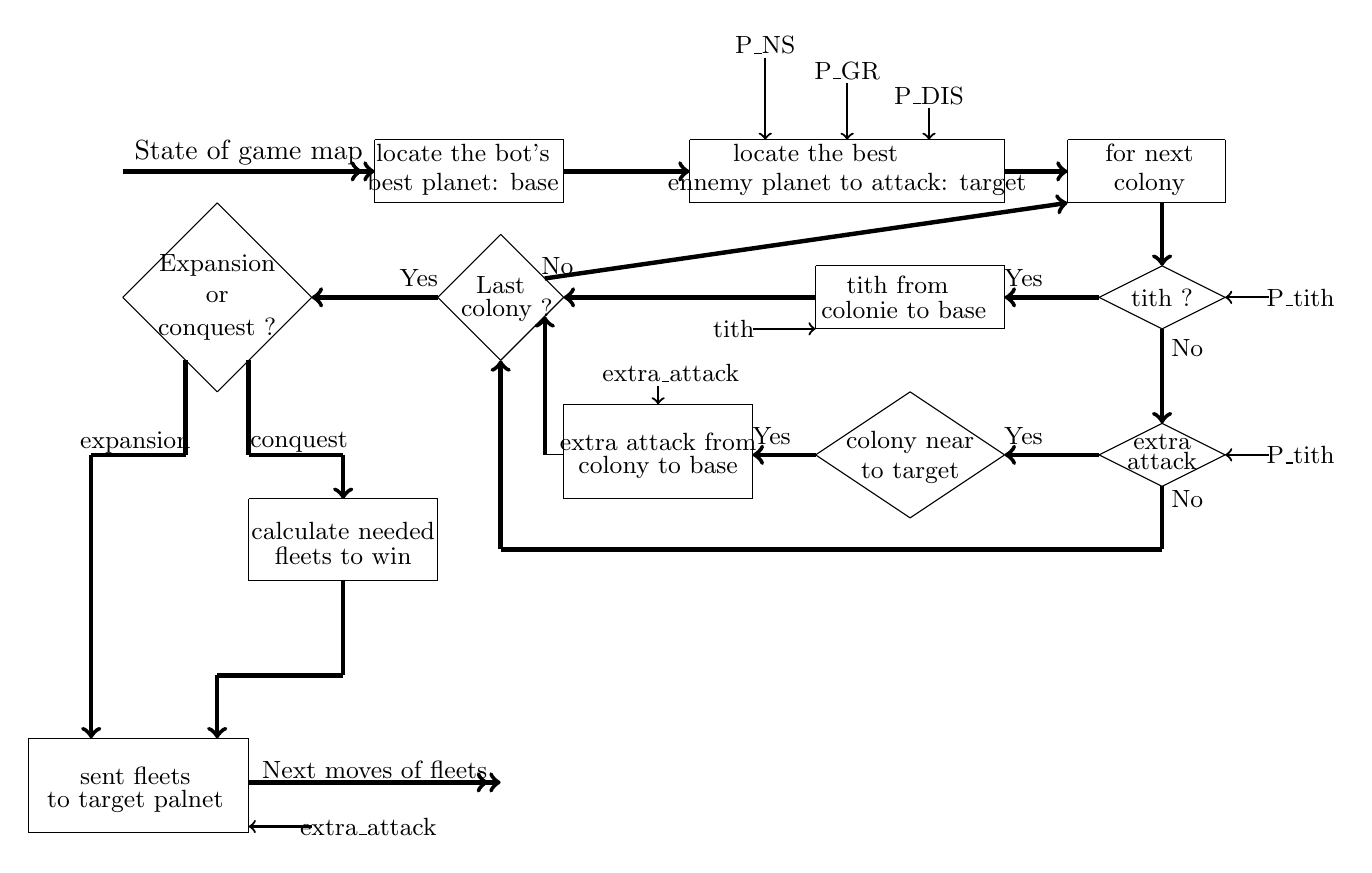
\begin{tikzpicture}[scale = 0.8]
\draw [->][ultra thick](-1,20) -- (3,20);
\draw [->][ultra thick](-1,20) -- (2.8,20);
\node at (1,20.3) {State of game map};
\draw (3,20.5) --(3,19.5);
\draw (3,20.5) --(6,20.5);
\draw (6,20.5) --(6,19.5);
\draw (6,19.5) --(3,19.5);
\draw [->][ultra thick](6,20) -- (8,20);
\node at (4.4,20.3) {\small locate the bot's};
\node at (4.4,19.8) {\small best planet: base};
\draw (8,20.5) --(8,19.5);
\draw (8,20.5) --(13,20.5);
\draw (13,20.5) --(13,19.5);
\draw (13,19.5) --(8,19.5);
\draw [->][thick](9.2,21.8) -- (9.2,20.5);
\draw [->][thick](10.5,21.4) -- (10.5,20.5);
\draw [->][thick](11.8,21) -- (11.8,20.5);
\node at (10,20.3) {\small locate the best};
\node at (9.2,22) {\small P\_NS};
\node at (10.5,21.6) {\small P\_GR};
\node at (11.8,21.2) {\small P\_DIS};
\node at (10.5,19.8) {\small ennemy planet to attack: target};
\draw [->][ultra thick](13,20) -- (14,20);
\draw (14,20.5) --(14,19.5);
\draw (14,20.5) --(16.5,20.5);
\draw (16.5,20.5) --(16.5,19.5);
\draw (16.5,19.5) --(14,19.5);
\node at (15.3,20.3) {\small for next};
\node at (15.3,19.8) {\small colony};
\draw [->][ultra thick](15.5,19.5) -- (15.5,18.5);
\draw (15.5,18.5) --(14.5,18);
\draw (14.5,18) --(15.5,17.5);
\draw (15.5,17.5) --(16.5,18);
\draw (16.5,18) --(15.5,18.5);
\draw [->][thick](17.2,18) -- (16.5,18);
\node at (17.7,18) {\small P\_tith};
\draw [->][thick](17.2,15.5) -- (16.5,15.5);
\node at (17.7,15.5) {\small P\_tith};
\node at (15.5,18) {\small tith ?};
\node at (15.5,15.7) {\small extra};
\node at (15.5,15.4) {\small attack};
\draw [->][ultra thick](15.5,17.5) -- (15.5,16);
\node at (15.9,17.2) {\small No};
\draw (15.5,16) --(14.5,15.5);
\draw (14.5,15.5) --(15.5,15);
\draw (15.5,15) --(16.5,15.5);
\draw (16.5,15.5) --(15.5,16);
\draw [->][ultra thick](14.5,18) -- (13,18);
\node at (13.3,18.3) {\small Yes};
\draw [ultra thick](15.5,15) -- (15.5,14);
\node at (15.9,14.8) {\small No};
\draw [ultra thick](15.5,14) -- (5,14);
\draw [->][ultra thick](5,14) -- (5,17);
\draw (13,18.5) --(13,17.5);
\draw (13,17.5) --(10,17.5);
\draw (10,17.5) --(10,18.5);
\draw (10,18.5) --(13,18.5);
\node at (13.3,15.8) {\small Yes};
\node at (11.3,18.2) {\small tith from};
\node at (11.4,17.8) {\small colonie to base};
\node at (8.7,17.5) {\small tith};
\draw [->][thick](9,17.5) -- (10,17.5);
\draw [->][ultra thick](14.5,15.5) -- (13,15.5);
\node at (9.3,15.8) {\small Yes};
\draw (13,15.5) --(11.5,16.5);
\draw (11.5,16.5) --(10,15.5);
\draw (10,15.5) --(11.5,14.5);
\draw (11.5,14.5) --(13,15.5);
\node at (11.5,15.7) {\small colony near};
\node at (11.5,15.2) {\small to target};
\draw [->][ultra thick](10,15.5) -- (9,15.5);
\draw (9,16.3) --(9,14.8);
\draw (9,14.8) --(6,14.8);
\draw (6,14.8) --(6,16.3);
\draw (6,16.3) --(9,16.3);
\node at (7.5,15.7) {\small extra attack from};
\node at (7.5,15.3) {\small colony to base};
\draw [->][thick](7.5,16.6) -- (7.5,16.3);
\node at (7.7,16.8) {\small extra\_attack};
\draw [->][ultra thick](10,18) -- (6,18);
\draw (6,18) --(5,19);
\draw (5,19) --(4,18);
\draw (4,18) --(5,17);
\draw (5,17) --(6,18);
\node at (5,18.2) {\small Last};
\node at (5.1,17.8) {\small colony ?};
\draw [->][ultra thick](5.7,18.3) -- (14,19.5);
\node at (5.9,18.5) {\small No};
\node at (3.7,18.3) {\small Yes};
\draw (6,15.5) -- (5.7,15.5);
\draw [->][ultra thick](5.7,15.5) -- (5.7,17.7);
\draw [->][ultra thick](4,18) -- (2,18);
\draw (2,18) -- (0.5,19.5);
\draw (0.5,19.5) -- (-1,18);
\draw (-1,18) -- (0.5,16.5);
\draw (0.5,16.5) -- (2,18);
\node at (0.5,18.5) {\small Expansion };
\node at (0.5,18) {\small or };
\node at (0.5,17.5) {\small conquest ?};
\draw [ultra thick](1,17) -- (1,15.5);
\draw [ultra thick](1,15.5) -- (2.5,15.5);
\node at (1.8,15.7) {\small conquest};
\draw [->][ultra thick](2.5,15.5) -- (2.5,14.8);
\draw (1,14.8) -- (4,14.8);
\draw (4,14.8) -- (4,13.5);
\draw (4,13.5) -- (1,13.5);
\draw (1,13.5) -- (1,14.8);
\node at (2.5,14.3) {\small calculate needed};
\node at (2.5,13.9) {\small fleets to win};
\draw [ultra thick](0,17) -- (0,15.5);
\draw [ultra thick](0,15.5) -- (-1.5,15.5);
\draw [->][ultra thick](-1.5,15.5) -- (-1.5,11);
\draw (-2.5,11) -- (1,11);
\draw (-2.5,9.5) -- (1,9.5);
\draw (-2.5,11) -- (-2.5,9.5);
\draw (1,11) -- (1,9.5);
\draw [ultra thick](2.5,13.5) -- (2.5,12);
\draw [ultra thick](2.5,12) -- (0.5,12);
\node at (-0.8,15.7) {\small expansion};
\draw [->][ultra thick](0.5,12) -- (0.5,11);
\node at (-0.8,10.4) {\small sent fleets};
\node at (-0.8,10) {\small to target palnet};
\draw [->][ultra thick](1,10.3) -- (4.8,10.3);
\draw [->][ultra thick](1,10.3) -- (5,10.3);
\node at (3,10.5) {\small Next moves of fleets};
\draw [->][thick](2,9.6) -- (1,9.6);
\node at (2.9,9.6) {\small extra\_attack};
\end{tikzpicture}
\caption{The states that are governing the behaviour of the AisBot including the parameters used on the evaluation of the bot's behaviour. these parameters will improve by the clonal selection algorithm (CLONALG).}
\end{figure*}

%If your manuscript has supplementary content you can also use the \verb"interact" class file to prepare all or part of it using the \verb"suppldata" document-class option, which will suppress the `article history' date. This option \emph{must not} be used on any primary content. Note that authors are solely responsible for the preparation of all supplemental material.

%%\includepdf[scale=0.7,pages=1]{botDiagram}


As we mentioned previously, the purpose of this study is to try to optimize the behaviour of a bot during the planet war RTS game. In order to improve our experimentation, we use the AisBot as a conquer bot in this game, and it works as follows: first of all, when a turn is started, the bot tries to determine the base planet based on a score function and the rest of planets are used as colonies.Secondly, the bot decides which planet to attack for the next turn or if it owns additional planet the action will be considered as a reinforcement, in order to reach the target planet, it can take some number of turns. If the bot trying to attack a target is owned by a neutral, the action will be considered as an expansion; however, if it's owned by the enemy, the action will be considered as a conquest. Once the base planet is reinforced by starships coming from colonies, the action will be considered as a Tith. In addition, when colonies that are closed to the target planet than the base is allowed to attack the target by sending fleets, instead of reinforcing the base and this one sends those fleets to the target planet, but move directly to the target. Besides, when a planet was targeted by the bot, it is no possible to decide another attack against the same planet until the first one finished, that is mean, for each fleet sent to perform an attack, it knows the target planet in its data structure. \\

In order to improve the behaviour of the bot,  a set of rules is defined included some parameters classified by weights, probabilities and amounts. the parameters signification is : 
\begin{itemize}
\item \textit{$Tith_{perc}$}: starships proportions that the bot can sends.
\item \textit{$Tith_{prob}$}: Tith probability that a colony sends to the base planet.
\item \textit{$w_{NS}$}: weight of starships number hosted on the planet.
\item \textit{$w_{DIS}$}: weight of distance between the base and the target planet.
\item \textit{$w_{GR}$}: weight of growth rate according to the target planet.
\item \textit{$Pool_{perc}$}: percentage of extra starships can send from the base to the target planet.
\item \textit{$Support_{perc}$}: Percentage of extra starships from the colony to the target.
\item \textit{$Support_{prob}$}: Probability of sending extra starships from the colony to the target.
\end{itemize}
Furthermore, each parameter takes some values during the optimization process depends on it meaning in the game, our conquer bot will be based on these values to make decisions during the game. To determine the target planet the bot will use a score function define as follow:

\begin{equation}
Score(p) = \frac{p.NumStarships.w_{NS-DIS}.Dist(base,p)}{1+p.GrowthRate.w_{GR}}
\end{equation}

Where the $w_{NS-dis}$ and the $w_{GR}$ are weights related successively to starships number, the growth rate for the planet and the distance to reach the target. As we mentioned above the $base$ is the planet which has the highest number of starships and $p$ refer to planet want to evaluate. \\ 

When the Tith and the attack process are performed by the colonies, the base planet also sends starships to attack the target. The number of starships sends to attack is estimated according to the attack mode, if the bot attack mode is expansion where the target does not generate starships during the game that implies the bot will integrate a very specific starships number to be able to defeat the planet target, on the other hand, if the bot attack mode is a conquest, the engine will estimate the number of troops needs to beat the enemy.
\section{AisBot: an AIS optimization}
The purpose of our optimization is to make the bot move faster and try to minimize the number of turns before destroying the enemy. On the other hand, a CLONALG algorithm will be applied in the set of parameters that will determine the behaviour of the bot, once the parameters are improved, the bot will upload them in order to go under real game scenarios. \\

Therefore, the purpose is to determine the parameters values in order to evaluate the bot's behaviour.The AIS proposed in this study use a floating array to represent all parameters defined previously, while, the clonal proliferation process works on a totally new array with a specific proliferation factor for each parameter according to its fitness. The maturation mechanism is applied to the cloned antibodies by mutating the parameters values using the equation (1) with a probability amount to minimize the bad antibodies. \\

The selection process based on an evaluation technic by implementing tournaments where each cloned individual used to compete with the aim of being selected for the next generation from the best results were chosen. The evaluation of an individual is staged by including their parameters for the AisBot behaviour and placing the bot on a real planet war game against the RandomBot on five maps. \\

The aim of this optimization is to minimize the number of turns needs to win, the best bot is the one that plays fewer turns until win; this kind of ranking bots strongly shown a constraint problem is that each individual was able to win every single game.\\

\section{Exprementation and results}
In order to improve the parameters used by the bot during the game, a CLONALG and PSO algorithms will be running in this purpose. 

To evaluate each parameter, the optimization process for the two algorithms will move as follow: 
first of all, for each individual in the initial population, it will run a real game match with the appropriate parameters values for 5 maps. Secondly, the parameters will evaluate according to the last results getting and repeatedly until the critical condition will be achieved; in our case is the generations and epochs factors.\\

\par The algorithms parameters can be found on the Table 1, Table 2 and Table 3 for CLONALG, PSO, and GA respectively:
\begin{table}[h!]
\centering
\begin{tabular}{ |c|c| }
\hline
 Parameters & Values \\ 
\hline
 Number of antibodies & 20 \\ 
 Number of generations & 15 \\  
 maximun antbodies Cloned & 72 \\ 
 \hline   
\end{tabular}
\centering
\caption{Parameters used in the CLONALG algorithm}
\label{TABLE 1}
\end{table}

\begin{table}[h!]
\centering
\begin{tabular}{ |c|c| }
\hline
 Parameters & Values \\ 
\hline
 Number of particles & 20 \\ 
 Epochs & 15 \\  
 Inertia & 0.73 \\
 Cognitive Component & 2 \\
 Social Component & 2 \\ 
 \hline   
\end{tabular}
\caption{Parameters used in the PSO algorithm}
\label{TABLE 2}
\end{table}

\begin{table}[h!]
\centering
\begin{tabular}{ |c|c| }
\hline
 Parameters & Values \\ 
\hline
 Number of individuals & 400 \\ 
 Mutation Probability & 0.02 \\  
 Crossover probability & 0.6 \\
 Replacement policy & 2-individuals elitism \\
 \hline   
\end{tabular}
\caption{Parameters used in the GA}
\label{TABLE 3}
\end{table}



The figure(5) represent the different maps played by the initial bot with the primary parameters values in the two optimization methods presented in this study. The blue color shows the AisBot and the black one is for the PSOBot before running the two algorithms. While the red and the green ones represent the AisBot and PSOBot respectively after the optimization of the parameters. On the other hand, Y-axis proves the number of turns played by each bot till winning the game. \\

\begin{comment}
\begin{figure}
\begin{center}
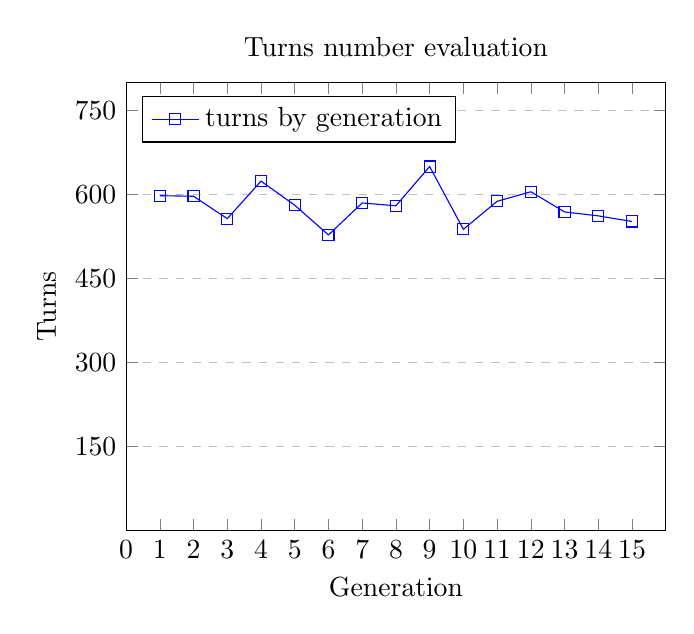
\begin{tikzpicture}
\begin{axis}[
    title={Turns number evaluation},
    xlabel={Generation},
    ylabel={Turns},
    xmin=0, xmax=16,
    ymin=0, ymax=800,
    xtick={0,1,2,3,4,5,6,7,8,9,10,11,12,13,14,15},
    ytick={150,300,450,600,750},
    legend pos=north west,
    ymajorgrids=true,
    grid style=dashed,
]
 
\addplot[
    color=blue,
    mark=square,
    ]
    coordinates {
    (1,598)(2,597)(3,557)(4,624)(5,581)(6,528)(7,585)(8,580)(9,650)(10,538)(11,588)(12,605)(13,569)(14,562)(15,552)
    };
    \legend{turns by generation}
 
\end{axis}
\end{tikzpicture}
\end{center}
\caption{the evaluation of the number of turns plays by the bot until win in 5 maps, and it appears that the number of turns needs to win in five maps decrease after the evaluation process}
\end{figure}
\end{comment}

\begin{figure}
\begin{center}
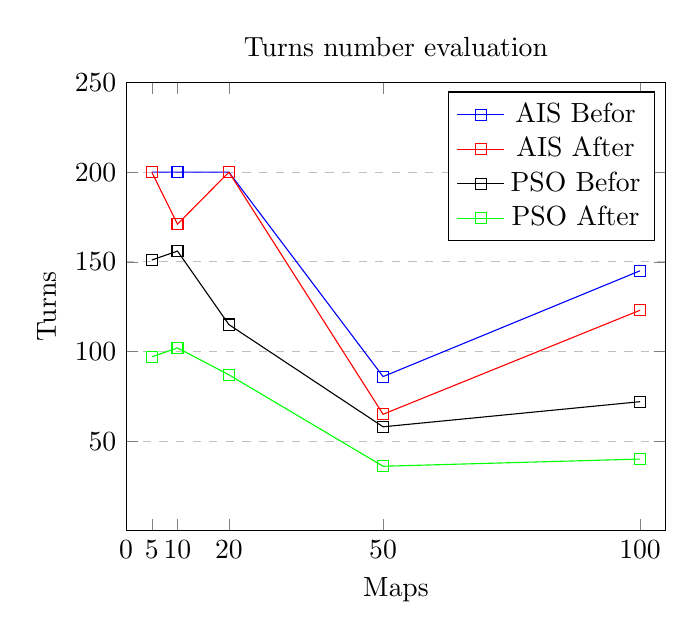
\begin{tikzpicture}
\begin{axis}[
    title={Turns number evaluation},
    xlabel={Maps},
    ylabel={Turns},
    xmin=0, xmax=105,
    ymin=0, ymax=250,
    xtick={0,5,10,20,50,100},
    ytick={50,100,150,200,250},
   % legend pos=outer north east,
    ymajorgrids=true,
    grid style=dashed,
]
 
\addplot[
    color=blue,
    mark=square,
    ]
    coordinates{(5,200)(10,200)(20,200)(50,86)(100,145)};
    
    \addplot[
    color=red,
    mark=square,
    ]
    coordinates{(5,200)(10,171)(20,200)(50,65)(100,123)};
    
    \addplot[
    color=black,
    mark=square,
    ]
    coordinates{(5,151)(10,156)(20,115)(50,58)(100,72)};
    
    \addplot[
    color=green,
    mark=square,
    ]
    coordinates{(5,97)(10,102)(20,87)(50,36)(100,40)};
    
    
    \legend{AIS Befor, AIS After, PSO Befor, PSO After}
 
\end{axis}
\end{tikzpicture}
\end{center}
\caption{The evaluation of the turns number needed to win around multiple maps between initial bot and optimized one using the AIS and PSO algorithms}
\end{figure}


Table 4 describes the initial parameters used by the bot in the several methods where the colonies have multiple strategies to send a Tith to the base planet according to the optimization algorithms; (0.78) as a high value used by the AISBot with a medium percentage to send starships to help the base. The GABot have a probability around (0.5) and to send a fewer number of starships which can be explained that each colony tries to protect itself. For the PSOBot we can see that the colonies have no high interest to help the base (0.19). On the other hand, the planet in all bots have a high probability to perform an attack (0.82, 0.96, 0.9) for AIS PSO and GA respectively with the minimum number of troops expect the GA with (50\%). Based on this, in each attack, the planet can send an extra number of the starships to defeat the enemy and that not interesting for the AISBot and GABot with (0.12, 0.25), while the PSOBot have a high percentage for this (0.78). Finally, to determine a target, the bot based on three parameters distance, growth rate and the number of starships where all bots have a high probability for the distance and growth rate factors; while the AISBot have a less interest about the number of starships (1\%).\\

Table(5) describe the parameters values after the optimization in different methods. As we can see the PSOBot increase the probability of each colony to send a reinforcement for the base planet (0.95) with a high number of troops. For the support probabilities, all the bot decrease the huge amount for performing an attack with (72\%) for PSOBot instead of (96\%). On the other side, all of the bots have a high interest to send extra starships in battles with the base (43\%) for AISBot, (64\%) for the PSOBot and (72\%) for the GABot. By the end, for the determination of the target planet, the AISBot take the number of starships as the effective factor(0.81) and decrease both the distance and the growth rate (0.26, 0.6)  as well as the PSOBot where take the number of starships as the highly effective factor(0.89). In the other side, the GABot decide to select the distance as the first factor that will be based on to determine their targets(84\%). \\

\begin{table}
\centering
\begin{tabular}{|c|c|c|c|}
\hline
 Parameter & AIS & PSO & GA \\ 
 \hline
 $Tith_{perc}$ & 0.505 & 0.606 & 0.1\\  
 \hline
 $Tith_{prob}$ & 0.778 & 0.192 & 0.5\\
 \hline
 $W_{NS}$ & 0.1 & 0.493 & 1\\
 \hline
 $W_{GR}$ & 0.933 & 0.554 & 1\\
 \hline
 $W_{DIS}$ & 0.562 & 0.835 & 1\\
 \hline
 $Pool_{perc}$ & 0.12 & 0.782 & 0.25\\
 \hline
 $Support_{perc}$ & 0.07 & 0.281 & 0.5\\
 \hline
 $Support_{prob}$ & 0.829 & 0.966 & 0.9\\
 \hline  
\end{tabular}
\caption{Parameters used by the initial bot befor runing the different optimization algorithms}
\label{TABLE 4}
\end{table}

\begin{table}
\centering
\begin{tabular}{|c|c|c|c|}
\hline
 Parameter & AIS & PSO & GA \\ 
 \hline
 $T_{perc}$ & 0.24 & 0.575 & 0.294\\  
 \hline
 $T_{prob}$ & 0.611 & 0.959 & 0.0389\\
 \hline
 $W_{NS}$ & 0.819 & 0.899 & 0.316\\
 \hline
 $W_{GR}$ & 0.6 & 0.159 & 0.316\\
 \hline
 $W_{DIS}$ & 0.262 & 0.478 & 0.844\\
 \hline
 $P_{perc}$ & 0.436 & 0.64 & 0.727\\
 \hline
 $S_{perc}$ & 0.504 & 0.015 & 0.822\\
 \hline
 $S_{prob}$ & 0.424 & 0.721 & 0.579\\
 \hline  
 %0.24,0.611,0.819,0.6,0.262,0.436,0.504,0.424
\end{tabular}
\caption{Parameters used by the optimized bot after the runing of the algorithms}
\label{TABLE 4}
\end{table}


%0.505,0.778,0.1,0.933,0.562,0.12,0.075,0.829
\begin{comment}
\begin{figure}
\begin{center}
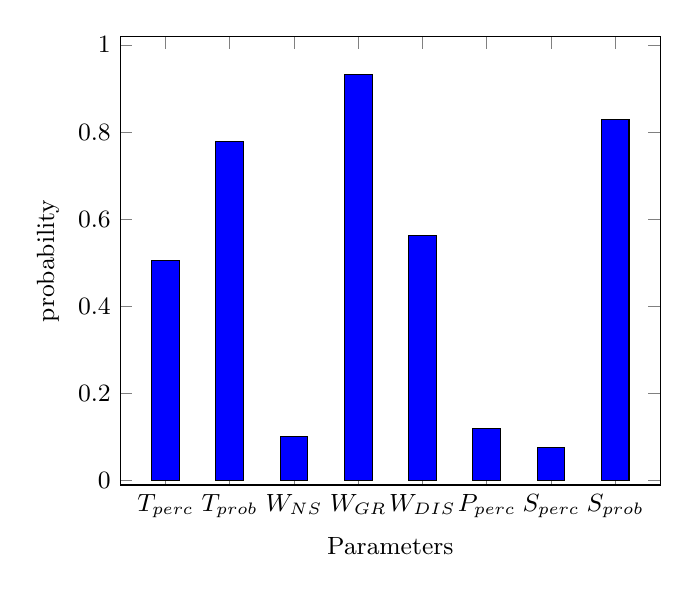
\begin{tikzpicture}[font=\small]
\begin{axis}[
    symbolic x coords={$T_{perc}$, $T_{prob}$, $W_{NS}$, $W_{GR}$, $W_{DIS}$, $P_{perc}$, $S_{perc}$, $S_{prob}$},
        ylabel = {probability},
        xlabel = {Parameters},
    xtick=data]
    \addplot[ybar,fill=blue] coordinates {
        ($T_{perc}$,0.505)
        ($T_{prob}$,0.778)
        ($W_{NS}$,0.1)
    ($W_{GR}$, 0.933)
    ($W_{DIS}$,0.562)
    ($P_{perc}$,0.12)
    ($S_{perc}$,0.075)
    ($S_{prob}$,0.829)
    };
\end{axis}
\end{tikzpicture}
\end{center}
\caption{The parameters values setting for the inital bot}
\end{figure}
\end{comment}
%0.24,0.611,0.819,0.6,0.262,0.436,0.504,0.424

\begin{comment}
\begin{figure}
\begin{center}
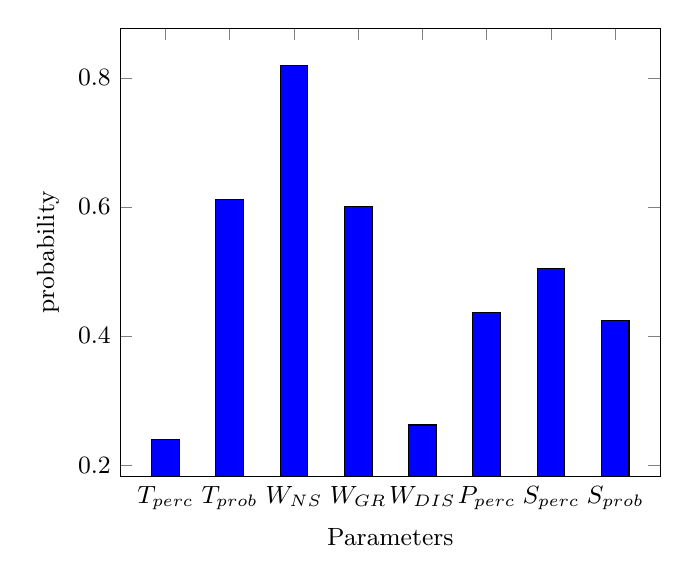
\begin{tikzpicture}[font=\small]
\begin{axis}[
    symbolic x coords={$T_{perc}$, $T_{prob}$, $W_{NS}$, $W_{GR}$, $W_{DIS}$, $P_{perc}$, $S_{perc}$, $S_{prob}$},
        ylabel = {probability},
        xlabel = {Parameters},
    xtick=data]
    \addplot[ybar,fill=blue] coordinates {
        ($T_{perc}$,0.24)
        ($T_{prob}$,0.611)
        ($W_{NS}$,0.819)
    ($W_{GR}$, 0.6)
    ($W_{DIS}$,0.262)
    ($P_{perc}$,0.436)
    ($S_{perc}$,0.504)
    ($S_{prob}$,0.424)
    };
\end{axis}
\end{tikzpicture}
\end{center}
\caption{The parameters values setting for the optimized bot}
\end{figure}
\end{comment}

\par
In general, figure (5) prove that the PSO algorithm gave the best results than the AIS CLONALG algorithm in many fields: 
\\
\begin{enumerate}
\item The time factor: in the algorithm structure we clearly constate that the AIS is more complex than the PSO where the CLONALG algorithm will evaluate all the initial population as the first step. After that, the next step is to clone and maturate all the proliferating individuals to another extended population (cloned population length > initial population length). Later, the algorithm will evaluate all the cloned population, replace and generate the new generation for the next generation evaluation. Instead of, in the PSO algorithm, each population will evaluate once in each iteration that will make the PSO faster than the AIS CLONALG. \\ 

\item The performance: in our case, the PSO algorithm results are more effective than the AIS ones and this can due to the algorithms shape. Furthermore, as we mentioned previously, the CLONALG algorithm needs to proliferate and mutate the initial population in order to increase the best elements within. In this stage, and according to the equation used for this purpose, the algorithm can accept less important element randomly initialized in the replacement step from the cloned to the evaluated population and they will be used in the next iteration. So, we can easily find inappropriate elements in the advanced steps of the algorithm and that will affect the algorithm performance. \\

\item In the mathematics point of view, the two algorithms used different types of equation:(a) the maturation equation in (1) used by the AIS algorithm which contains one factor is the scale factor k that can diverge the values from the optimum solution if it will take a random range of values. (b) in the PSO algorithm, the next move for every particle in the swarm will be based not only for self-evaluation(Pbest) but according to the whole swarm(Gbest) position in the working space and that what makes the elements converge repeatedly to the optimum solution in each iteration.
\end{enumerate}

\section{conclusions}
The conception of intelligent agents is the hardest task in the RTS games accordingly to the real-time aspect. This study aims to contribute to this growing area of research by exploring three different optimization methods to investigate the performance of the evolutionary algorithm under real problems. The optimization methods proceed in a parametrize space area in order to improve the general behavior of the agents. However, the investigation of the results showed the top hand of the EAs agents against the hand-coded ones, when the EAs bots can defeat all enemies in different situations using multiple improving algorithms in the less number of turns.

\bibliography{references}

\addcontentsline{toc}{section}{Bibliography}

\bibliographystyle{abbrv}

\end{document}
